\chapter{Estruturas de Dados para Inteiros}

Neste capítulo, voltamos ao problema de implementar um #SSet#.
A diferença agora é que assumimos que os elementos armazenados no #SSet# são inteiros com #w#-bits. Ou seja, queremos implementar #add(x)#, #remove(x)#, e #find(x)# onde $#x#\in\{0,\ldots,2^{#w#}-1\}$. Não é muito difícil	pensar em muitas aplicações em que os dados --- ou pelo menos a chave que usamos para classificar os dados --- é um número inteiro.

Discutiremos três estruturas de dados, cada uma com base nas idéias da anterior. A primeira estrutura, a #BinaryTrie# executa todas as três operações de um #SSet# em um tempo $O(#w#)$. Isso não é muito impressionante, pois qualquer subconjunto de $\{0,\ldots,2^{#w#}-1\}$ tem o tamanho $#n#\le 2^{#w#}$, para que $\log #n# \le #w#$. Todas as outras implementações de #SSet# discutidas neste livro realizam todas as operações em um tempo $O(\log #n#)$, para que sejam todas pelo menos tão rápidas quanto uma #BinaryTrie#.

A segunda estrutura, a #XFastTrie#, acelera a pesquisa em uma
#BinaryTrie# usando hashing. Com esse aumento de velocidade, a operação #find(x)# é executada em um tempo $O(\log #w#)$. No entanto, as operações #add(x)# e #remove(x)# em uma #XFastTrie# ainda levam um tempo $O(#w#)$ e o espaço usado por uma #XFastTrie# é $O(#n#\cdot#w#)$.

A terceira estrutura de dados, #YFastTrie#, usa uma #XFastTrie# para armazenar apenas uma amostra de aproximadamente um de cada $#w#$ elementos e armazena os elementos restantes em uma estrutura #SSet# padrão. Este truque reduz o tempo de execução de #add(x)# e #remove(x)# para $O(\log #w#)$ e diminui o espaço para $O(#n#)$.

As implementações usadas como exemplos neste capítulo podem armazenar qualquer tipo de dados, desde que um inteiro possa ser associado a eles. Nos exemplos de código, a variável #ix# é sempre o valor inteiro associado a #x#, e o método \javaonly{#in.#}#IntValue(x)# converte #x# em seu inteiro associado. No texto, entretanto, iremos simplesmente tratar #x# como se fosse um inteiro.

\section{#BinaryTrie#: Uma árvore de busca digital}
\seclabel{binarytrie}

\index{BinaryTrie@#BinaryTrie#}%
Uma #BinaryTrie# codifica um conjunto de inteiros de #w# bits em uma árvore binária.
Todas as folhas da árvore têm profundidade #w# e cada número inteiro é codificado como um caminho da raiz para a folha. O caminho para o inteiro #x# vira à esquerda no nível #i# se o #i#ésimo bit mais significativo de #x# é um 0 e vira à direita se for 1. \figref{binarytrie-ex} mostra um exemplo para o caso $#w#=4$, no qual a trie armazena os inteiros 3(0011), 9(1001), 12(1100) e 13(1101).
\begin{figure}
  \begin{center}
    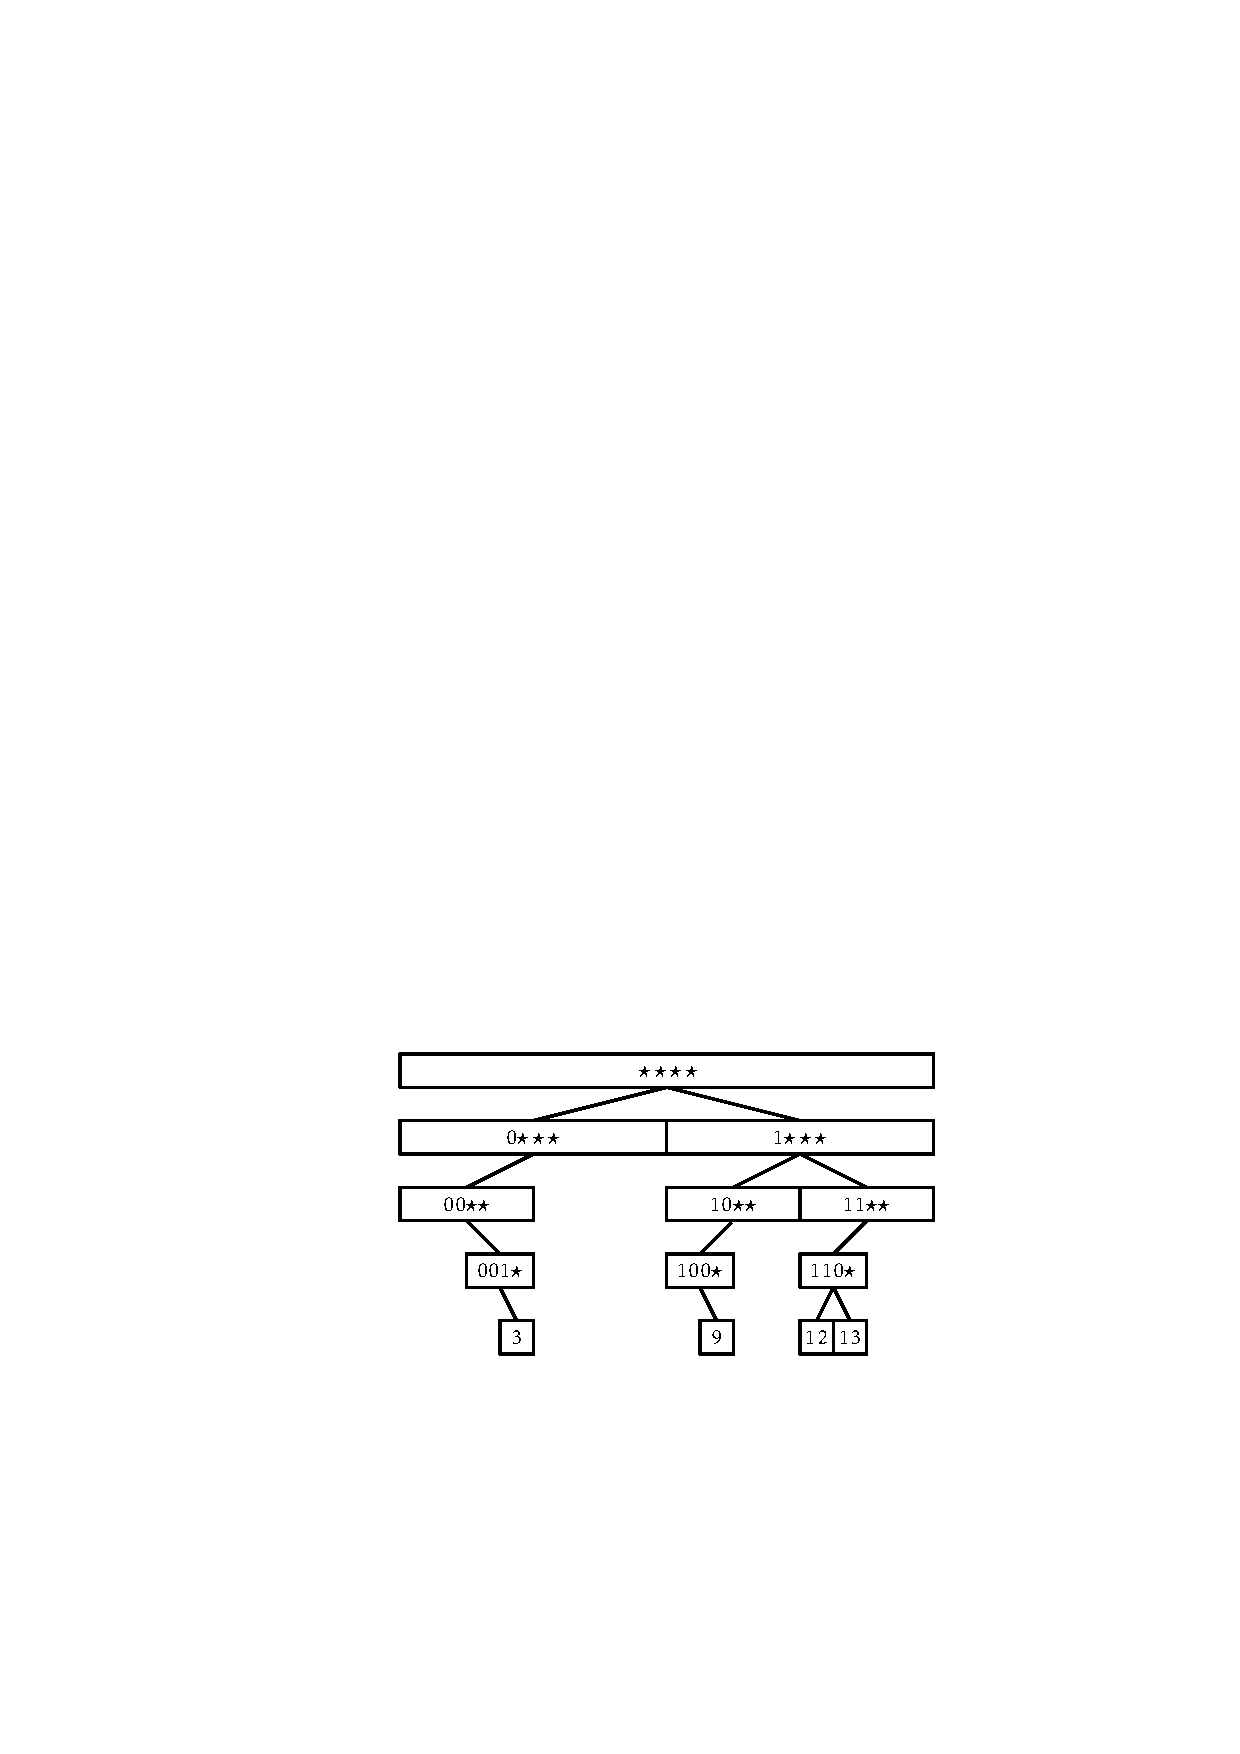
\includegraphics[width=\ScaleIfNeeded]{figs/binarytrie-ex-1}
  \end{center}
  \caption{Os inteiros armazenados em uma trie binária são codificados como caminhos da raiz para a folha.}
  \figlabel{binarytrie-ex}
\end{figure}

Como o caminho de pesquisa 
\index{caminho de pesquisa!em uma #BinaryTrie#}% 
para um valor #x# depende dos bits de #x#, será útil nomear os filhos de um nó, #u#, #u.child[0]# (#left#) e #u.child[1]# (#right#). Essas referências para os filhos na verdade servirão para dupla função. Como as folhas em uma trie binária não têm filhos, as referências são usadas para amarrar as folhas em uma lista duplamente encadeada.
Para uma folha na trie binária #u.child[0]# (#prev#) é o nó que vem antes de #u# na lista e #u.child[1]# (#next#) é o nó que segue #u# na lista. Um nó especial, #dummy#, é usado antes do primeiro nó e depois do último nó da lista (ver \secref{dllist}).
\cpponly {Nos exemplos de código, #u.child[0]#, #u.left# e #u.prev# referem-se ao mesmo campo no nó #u#, assim como #u.child[1]#, #u.right# e #u.next#.}

Cada nó, #u#, também contém um ponteiro adicional #u.jump#. Se o filho esquerdo de #u# estiver faltando, então #u.jump# aponta para a menor folha na subárvore de #u#. Se o filho direito de #u# estiver faltando, #u.jump# aponta para a maior folha na subárvore de #u#. Um exemplo de #BinaryTrie#, mostrando ponteiros #jump#  e a lista duplamente encadeada nas folhas, é mostrado na \figref{binarytrie-ex2}.

\begin{figure}
  \begin{center}
    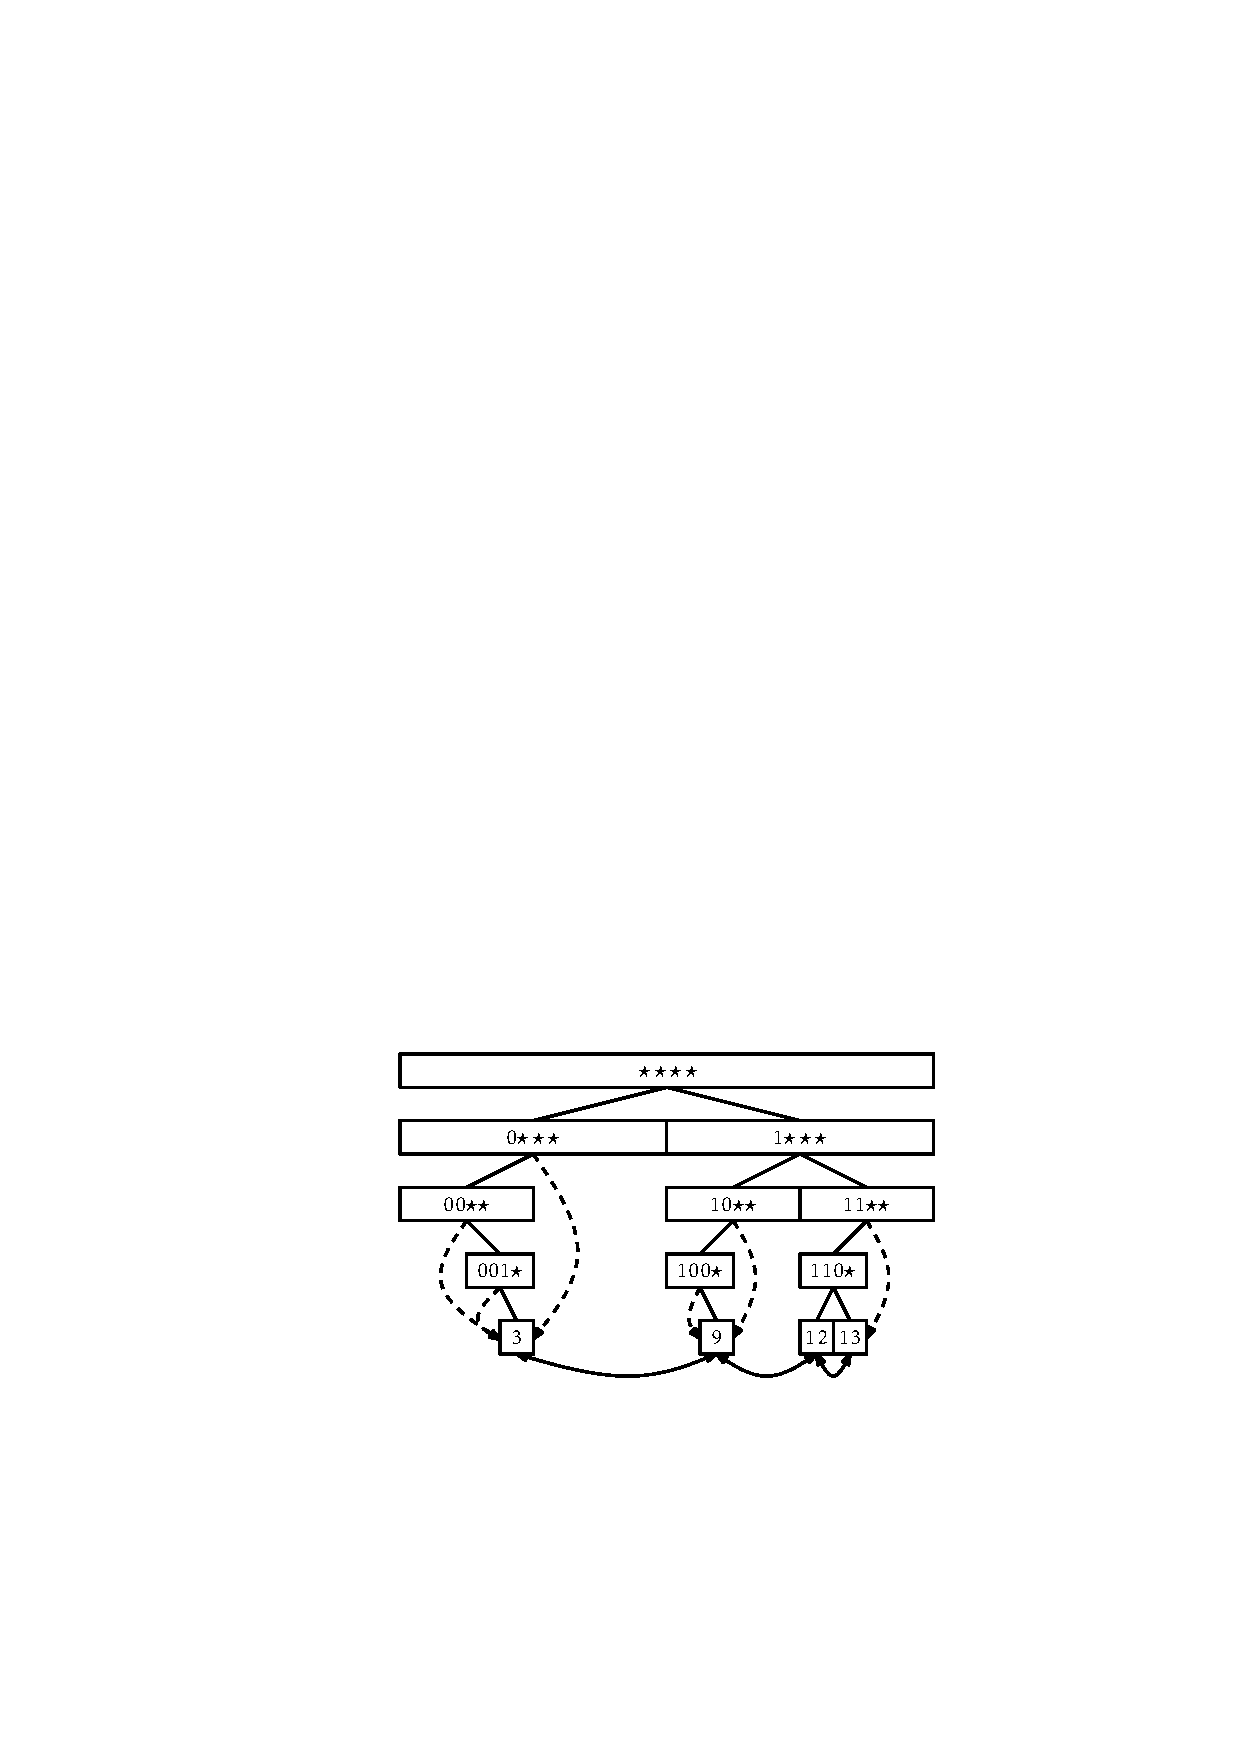
\includegraphics[width=\ScaleIfNeeded]{figs/binarytrie-ex-2}
  \end{center}
  \caption[A BinaryTrie]{Uma #BinaryTrie# com ponteiros #jump#  mostrados como arestas tracejadas curvas.}
  \figlabel{binarytrie-ex2}
\end{figure}


%\jxavaimport{ods/BinaryTrie.Node<Node}
%\cxppimport{ods/BinaryTrie.BinaryTrieNode<Node}

A operação #find(x)# em uma #BinaryTrie# é bastante simples.
Tentamos seguir o caminho de pesquisa de #x# na trie. Se chegarmos a uma folha, encontramos #x#. Se chegarmos a um nó #u# onde não podemos prosseguir (porque #u# está faltando um filho), seguimos #u.jump#, que nos leva à menor folha maior que #x# ou à maior folha menor que #x#. Qual desses dois casos ocorre depende se em #u# está faltando seu filho esquerdo ou direito, respectivamente. No primeiro caso (em #u# está faltando seu filho esquerdo), encontramos o nó que desejamos. No último caso (em #u# está faltando seu filho direito), podemos usar a lista encadeada para chegar ao nó que desejamos. Cada um desses casos é ilustrado em \figref{binarytrie-find}.
\codeimport{ods/BinaryTrie.find(x)}
\begin{figure}
  \begin{center}
    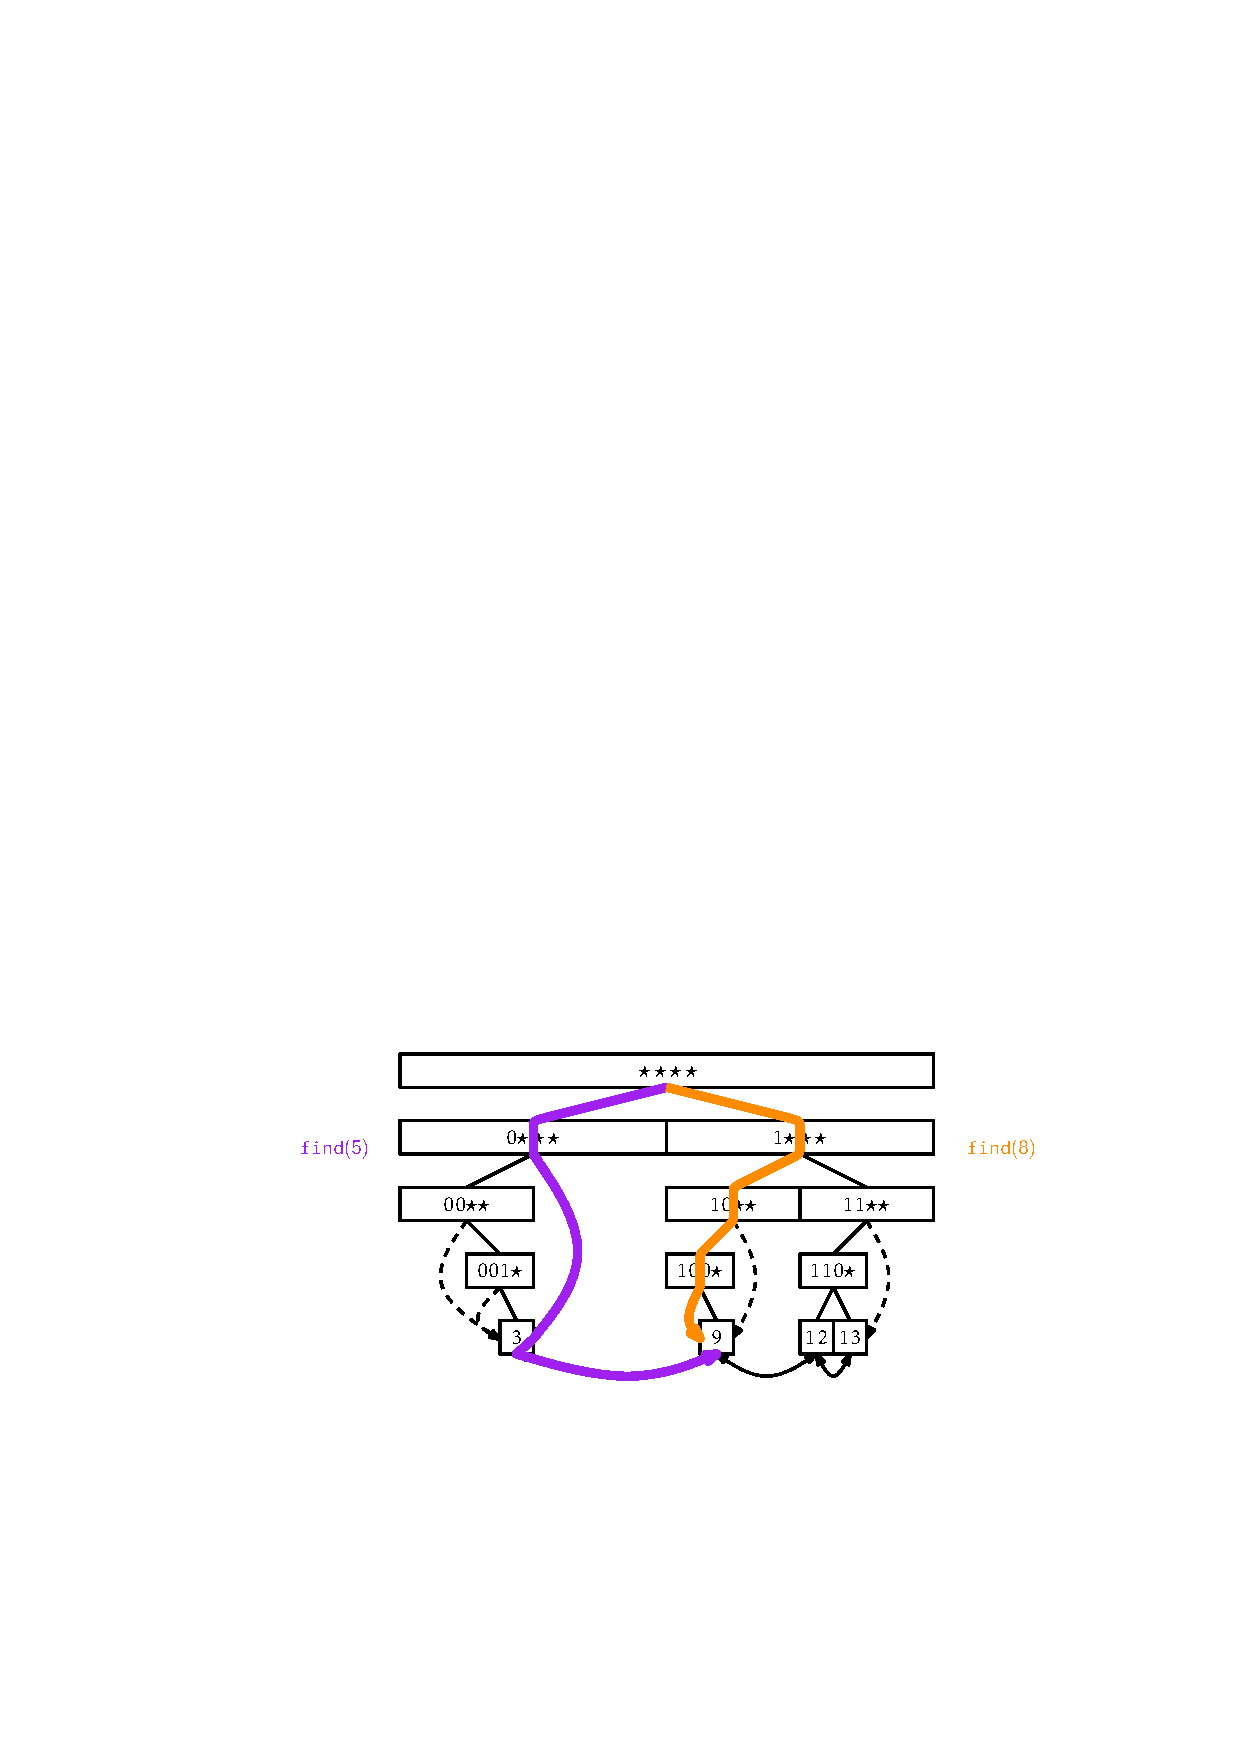
\includegraphics[width=\ScaleIfNeeded]{figs/binarytrie-ex-3}
  \end{center}
  \caption[Caminhos de pesquisa em uma BinaryTrie] {Os caminhos seguidos por #find(5)# e #find(8)#.}
  \figlabel{binarytrie-find}
\end{figure}
O tempo de execução do método #find(x)# é dominado pelo tempo que leva para seguir um caminho da raiz para a folha, então ele é executado em tempo $O(#w#)$.

A operação #add(x)# em uma #BinaryTrie# também é bastante simples, mas tem muito trabalho a fazer:
\begin{enumerate}
  \item Ele segue o caminho de busca por #x# até chegar a um nó #u# onde não pode mais prosseguir.
  \item Ele cria o restante do caminho de pesquisa de #u# para uma folha que contém #x#.
  \item Ele adiciona o nó, #u'#, contendo #x# à lista encadeada de folhas (tem acesso ao predecessor, #pred#, de #u'# na lista encadeada do ponteiro #jump# do último nó, #u#, encontrado durante a etapa~1.)
  \item Ele caminha de volta no caminho de pesquisa para #x#, ajustando os ponteiros #jump# nos nós cujo ponteiro de #jump# deve agora apontar para #x#.
\end{enumerate}
Uma adição é ilustrada na \figref{binarytrie-add}.
\begin{figure}
  \begin{center}
    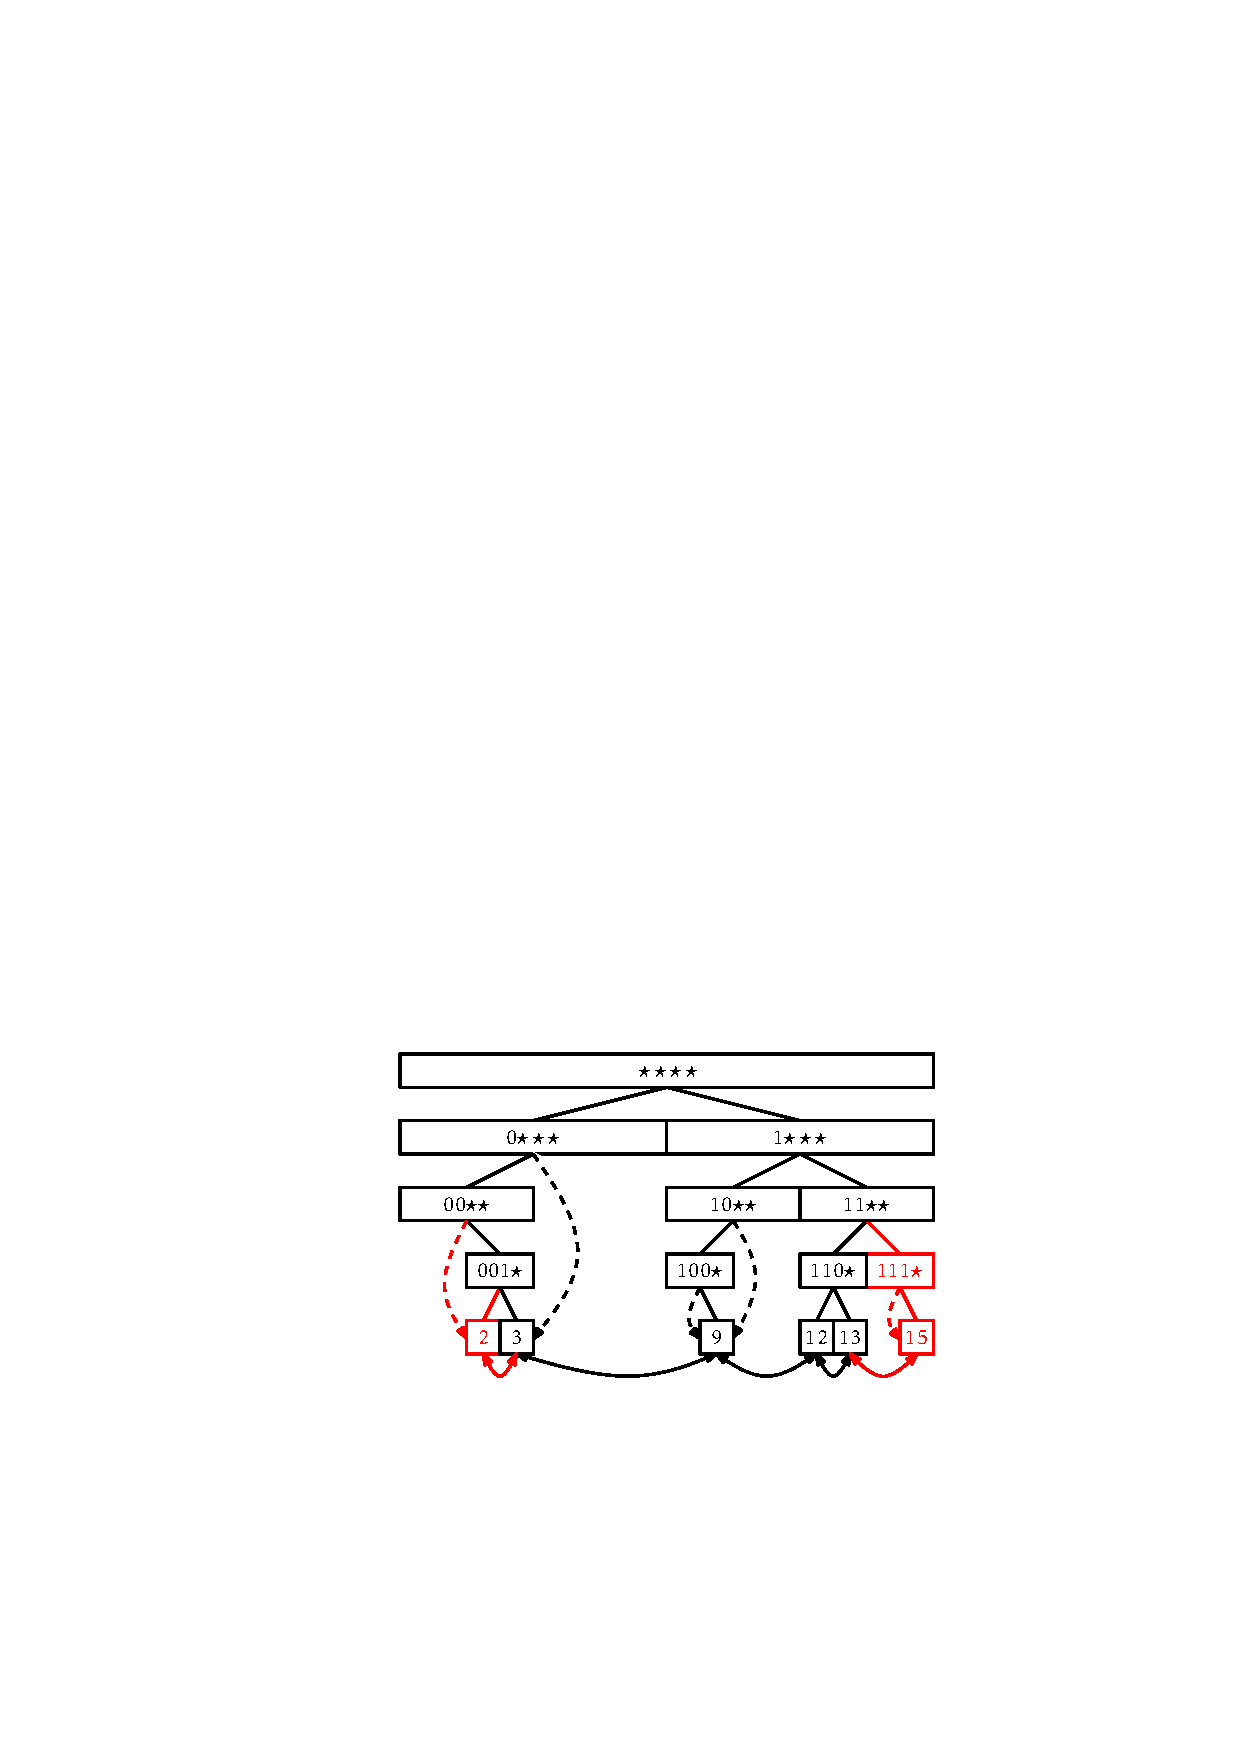
\includegraphics[width=\ScaleIfNeeded]{figs/binarytrie-add}
  \end{center}
  \caption[Adicionando a uma BinaryTrie] {Adicionando os valores 2 e 15 à #BinaryTrie# na
  \figref{binarytrie-ex2}.}
  \figlabel{binarytrie-add}
\end{figure}
\codeimport{ods/BinaryTrie.add(x)}
Este método executa uma caminhada pelo caminho de pesquisa de #x# e uma caminhada de volta para cima. Cada etapa dessas caminhadas leva um tempo constante, portanto o método #add(x)# é executado em um tempo $O(#w#)$.

A operação #remove(x)# desfaz o trabalho de #add(x)#. Como #add(x)#, ele tem muito trabalho a fazer:
\begin{enumerate}
  \item Segue o caminho de busca por #x# até chegar à folha, #u#, que contém #x#.
  \item Ele remove #u# da lista duplamente encadeada.
  \item Ele exclui #u# e, em seguida, retorna ao caminho de pesquisa de #x# excluindo nós até chegar a um nó #v# que tem um filho que não está no caminho de pesquisa de #x#.
  \item Ele sobe de #v# para a raiz, atualizando quaisquer ponteiros #jump# que apontam para #u#.
\end{enumerate}
Uma remoção é ilustrada na \figref{binarytrie-remove}.
\begin{figure}
  \begin{center}
    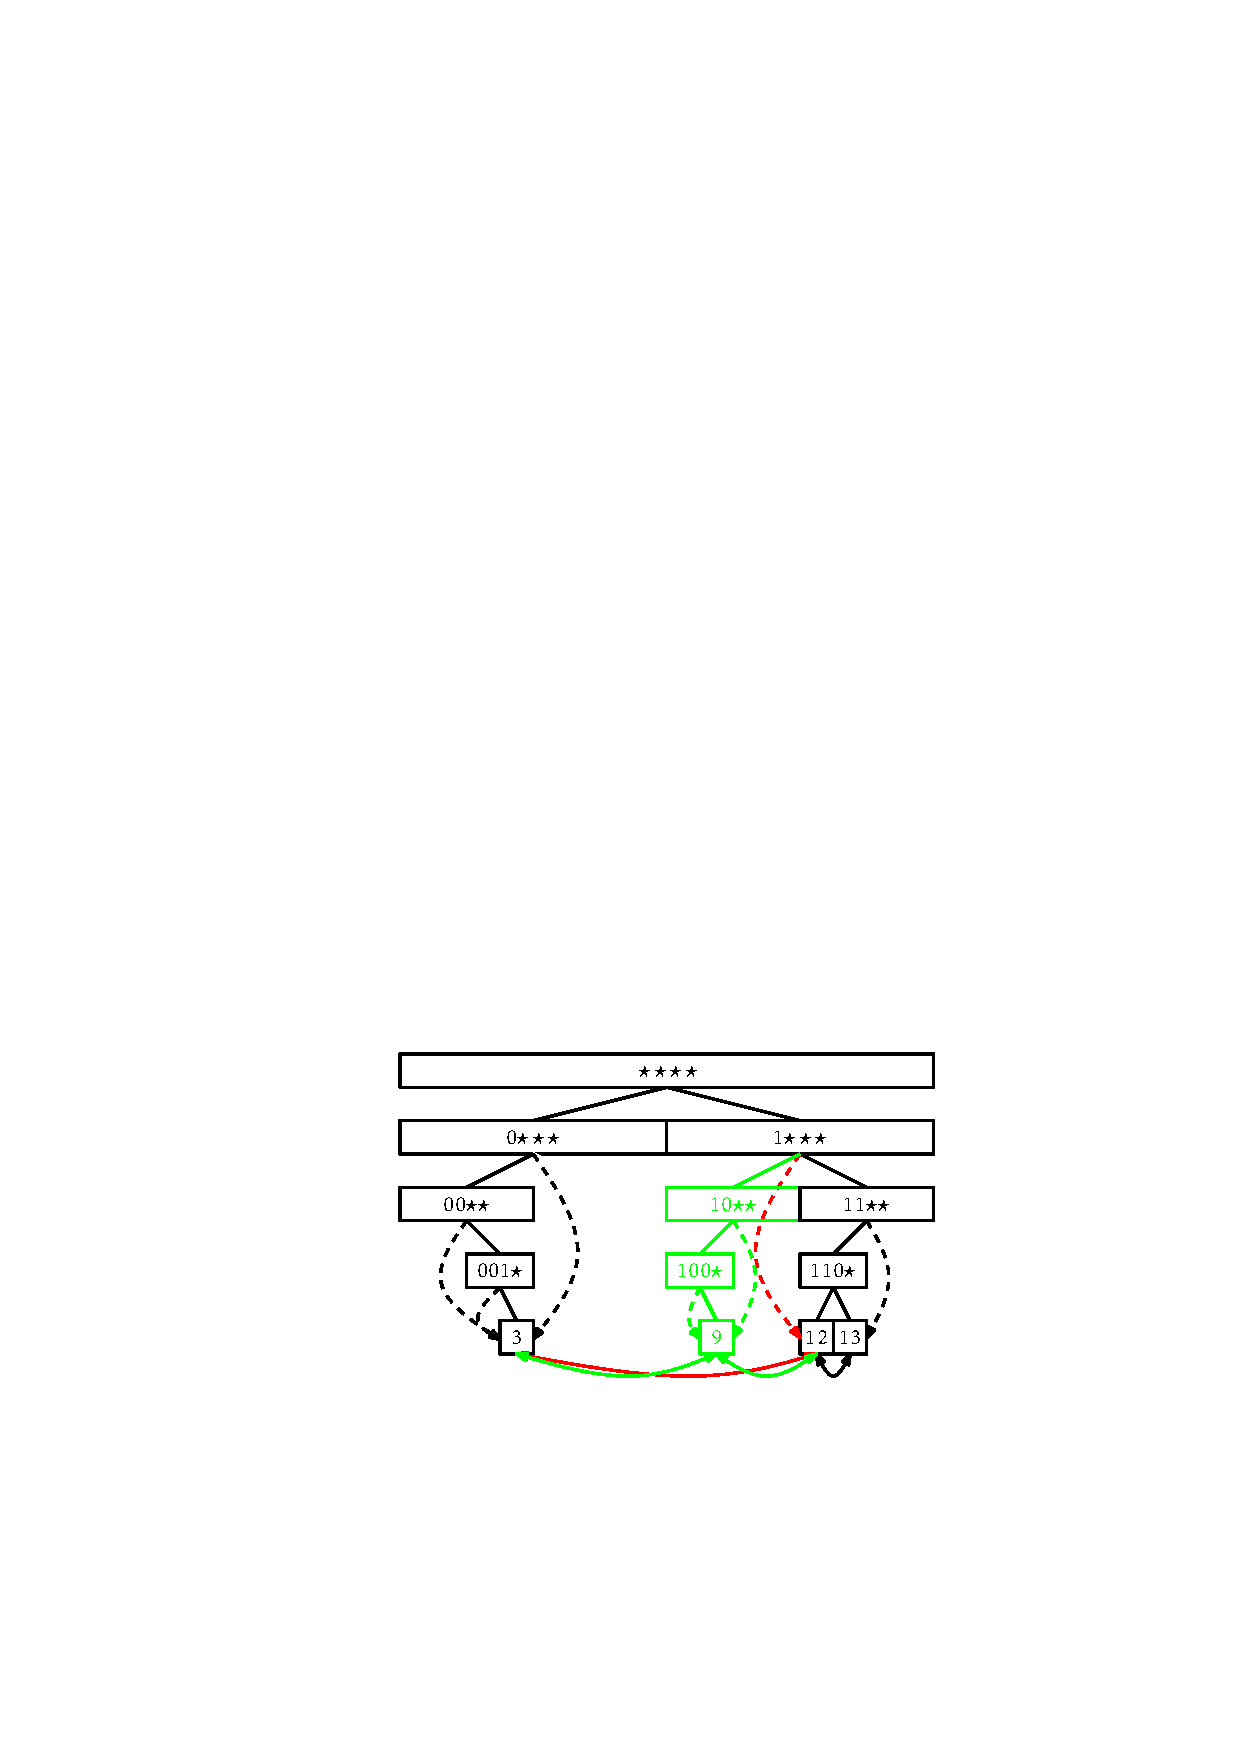
\includegraphics[scale=0.90909]{figs/binarytrie-remove}
  \end{center}
  \caption[Removendo de uma BinaryTrie]{Removendo o valor 9 da #BinaryTrie# na
  \figref{binarytrie-ex2}.}
  \figlabel{binarytrie-remove}
\end{figure}
\codeimport{ods/BinaryTrie.remove(x)}

\begin{thm}
Uma #BinaryTrie# implementa a interface #SSet# para inteiros de #w#-bits. Uma #BinaryTrie# suporta as operações #add(x)#, #remove(x)# e #find(x)# em um tempo $O(#w#)$ por operação. O espaço usado por uma #BinaryTrie# que armazena #n# valores é $O(#n#\cdot#w#)$.
\end{thm}

\section{#XFastTrie#: Pesquisando em tempo duplamente logarítmico}
\seclabel{xfast}

\index{XFastTrie@#XFastTrie#}%
O desempenho da estrutura #BinaryTrie# não é muito impressionante.
O número de elementos, #n#, armazenados na estrutura é no máximo $2^{#w#}$, então $\log #n#\le #w#$. Em outras palavras, qualquer uma das estruturas #SSet# baseadas em comparação descritas em outras partes deste livro são pelo menos tão eficientes quanto #BinaryTrie# e não estão restritas a armazenar apenas inteiros.

Em seguida, descrevemos a #XFastTrie#, que é apenas uma #BinaryTrie# com #w+1# tabelas hash --- uma para cada nível do teste. Essas tabelas hash são usadas para acelerar a operação #find(x)# para um tempo $O(\log #w#)$.
Lembre-se de que a operação #find(x)# em uma #BinaryTrie# está quase completa quando alcançamos um nó, #u#, onde o caminho de pesquisa para #x# gostaria de prosseguir para #u.right# (ou #u.left#) mas #u# não tem filho direito (respectivamente, esquerdo). Neste ponto, a pesquisa usa #u.jump# para pular para uma folha, #v#, da #BinaryTrie# e retornar #v# ou seu sucessor na lista encadeada de folhas. Uma #XFastTrie# acelera o processo de pesquisa usando a pesquisa binária
\index{pesquisa binária}%
nos níveis da trie para localizar o nó #u#.

Para usar a pesquisa binária, precisamos determinar se o nó #u# que estamos procurando está acima de um determinado nível, #i#, ou se #u# está no nível ou abaixo do #i#. Esta informação é fornecida pelos bits #i# de ordem mais alta na representação binária de #x#; esses bits determinam o caminho de pesquisa que #x# leva da raiz ao nível #i#. Para um exemplo, consulte \figref{xfast-path}; nesta figura, o último nó, #u#, no caminho de pesquisa para 14 (cuja representação binária é 1110) é o nó rotulado $11{\star\star}$ no nível 2 porque não há nenhum nó rotulado $111{\star}$ no nível 3. Portanto, podemos rotular cada nó no nível #i# com um número inteiro de #i# bits. Então, o nó #u# que estamos procurando estaria no nível #i# ou abaixo se e somente se houvesse um nó no nível #i# cujo rótulo corresponda aos bits #i# de ordem mais alta de #x#.

\begin{figure}
  \begin{center}
    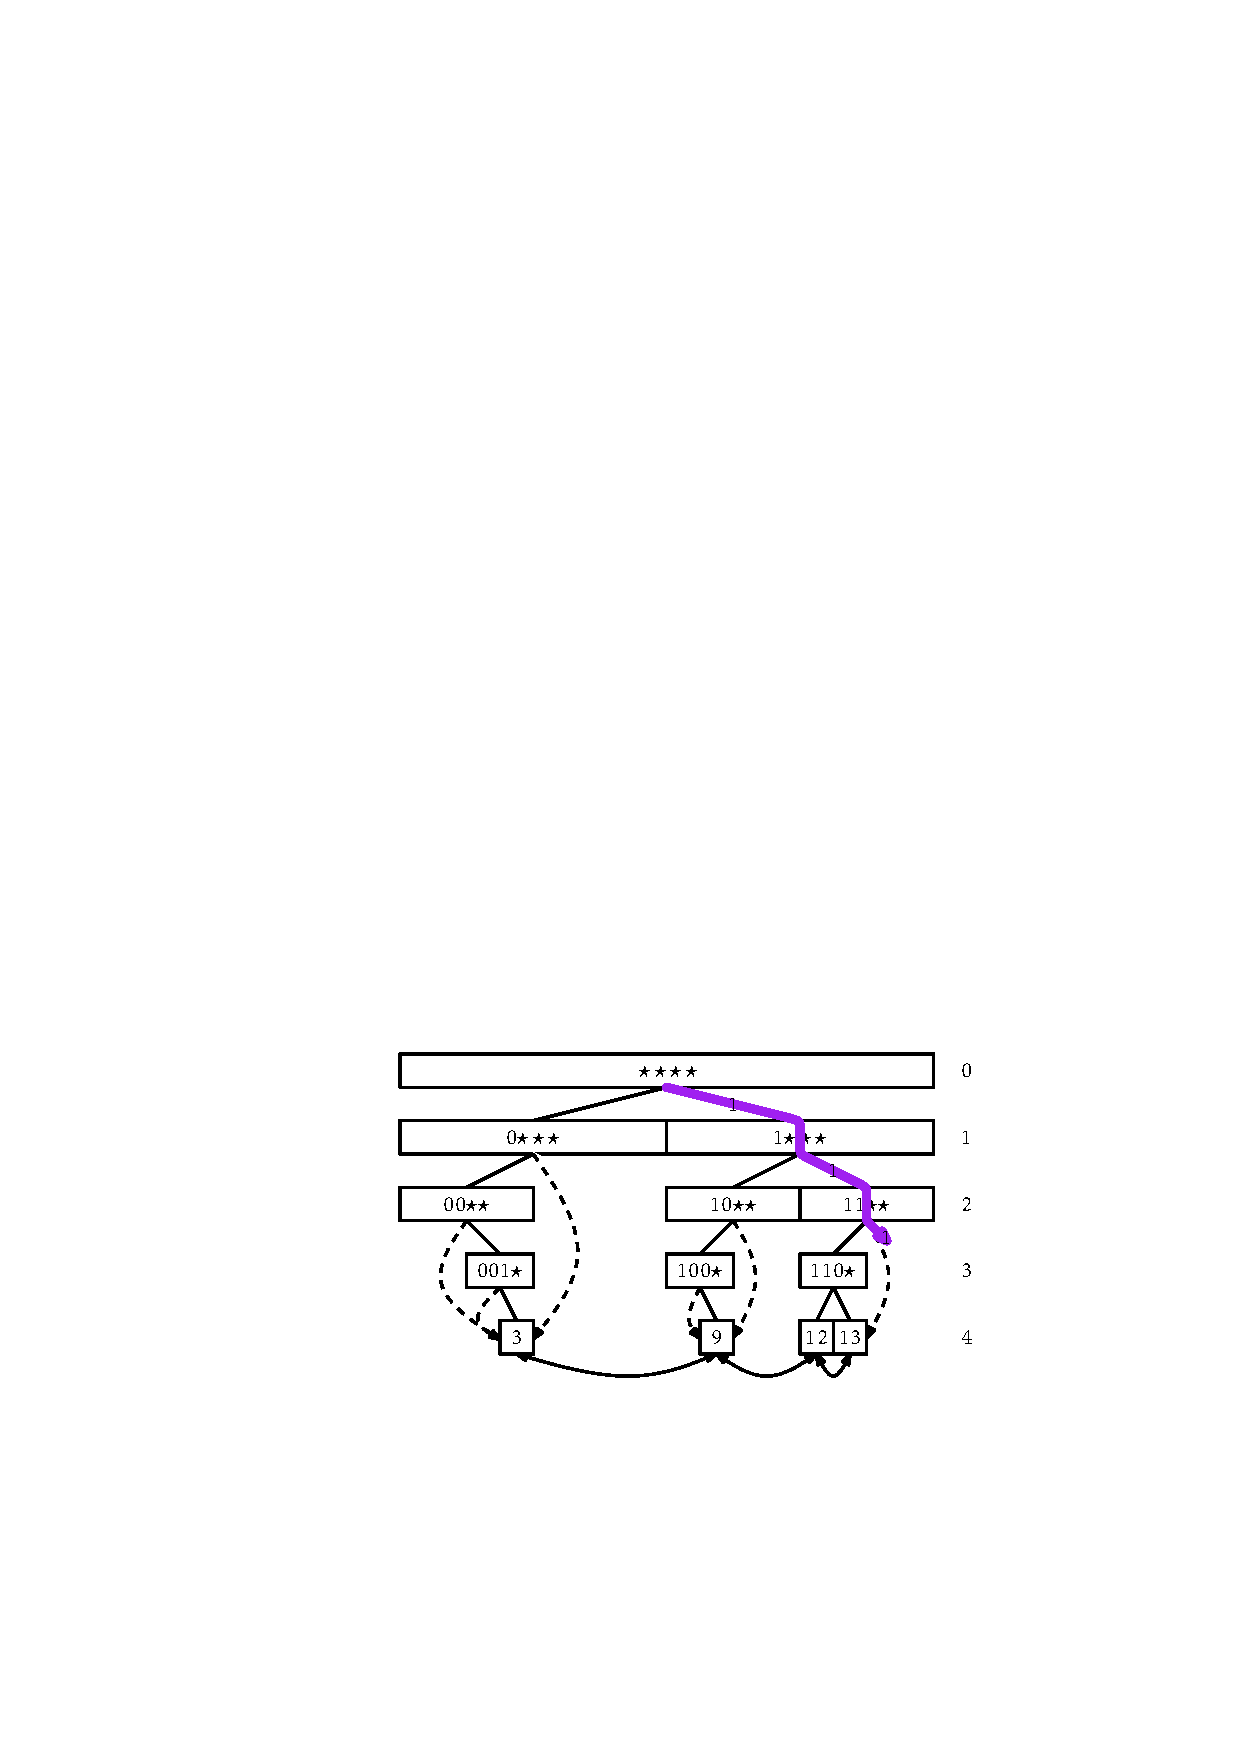
\includegraphics[scale=0.90909]{figs/xfast-path}
  \end{center}
  \caption{Como não há nenhum nó rotulado como $111\star$, o caminho de pesquisa para 14 (1110) termina no nó rotulado $11{\star\star}$.}
  \figlabel{xfast-path}
\end{figure}

Em uma #XFastTrie#, armazenamos, para cada $#i#\in\{0,\ldots,#w#\}$, todos os nós no nível #i# em um #USet#, #t[i]#, que é implementado como uma tabela hash (\chapref{hashing}). Usar este #USet# nos permite verificar em tempo esperado constante se há um nó no nível #i# cujo rótulo corresponde aos bits #i# de ordem mais alta de #x#. Na verdade, podemos até encontrar este nó usando
\javaonly{#t[i].find(x>>>(w-i))#}%
\cpponly{#t[i].find(x>>(w-i))#}%
\pcodeonly{#t[i].find(x>>(w-i))#}%

As tabelas de hash $#t[0]#,\ldots,#t[w]#$ nos permitem usar a pesquisa binária para encontrar #u#. Inicialmente, sabemos que #u# está em algum nível #i# com $0\le #i#<#w#+1$. Portanto, inicializamos $#l#=0$ e $#h#=#w#+1$ e repetidamente olhamos para a tabela hash #t[i]#, onde $#i#=\lfloor(#l+h#)/2\rfloor$. Se $#t[i]#$ contém um nó cujo rótulo corresponde aos bits #i# de ordem superior de #x#, então definimos #l=i# (#u# está no nível ou abaixo de #i#); caso contrário, definimos #h=i# (#u# está acima do nível #i#). Este processo termina quando $#h-l#\le 1$, caso em que determinamos que #u# está no nível #l#. Em seguida, completamos a operação #find(x)# usando #u.jump# e a lista duplamente encadeada de folhas.
\codeimport{ods/XFastTrie.find(x)}
Cada iteração do loop #while# no método acima diminui #h-l# por aproximadamente um fator de dois, então este loop encontra #u# após $O(\log #w#)$ iterações. Cada iteração executa uma quantidade constante de trabalho e uma operação #find(x)# em um #USet#, que leva um tempo esperado constante. O trabalho restante leva apenas um tempo constante, portanto o método #find(x)# em uma #XFastTrie# leva apenas um tempo esperado de $O(\log #w#)$.

Os métodos #add(x)# e #remove(x)# para uma #XFastTrie# são quase idênticos aos mesmos métodos em uma #BinaryTrie#. As únicas modificações são para gerenciar as tabelas hash #t[0]#,\ldots,#t[w]#. Durante a operação #add(x)#, quando um novo nó é criado no nível #i#, este nó é adicionado a #t[i]#. Durante uma operação #remove(x)#, quando um nó é removido do nível #i#, este nó é removido de #t[i]#. Como adicionar e remover de uma tabela hash leva um tempo esperado constante, isso não aumenta os tempos de execução de #add(x)# e #remove(x)# por mais de um fator constante. Omitimos uma listagem de código para #add(x)# e #remove(x)#, pois o código é quase idêntico à (longa) listagem de código já fornecida para os mesmos métodos em uma #BinaryTrie#.

O teorema a seguir resume o desempenho de uma #XFastTrie#:

\begin{thm}
Uma #XFastTrie# implementa a interface #SSet# para inteiros com #w#-bits. Uma #XFastTrie# suporta as operações
\begin{itemize}
\item #add(x)# e #remove(x)# em tempo esperado de $O(#w#)$ por operação e
\item #find(x)# em tempo esperado de $O(\log #w#)$ por operação.
\end{itemize}
O espaço usado por uma #XFastTrie# que armazena #n# valores é $O(#n#\cdot#w#)$.
\end{thm}

\section{#YFastTrie#: Um #SSet# de tempo duplamente logarítmico}
\seclabel{yfast}

A #XFastTrie# é uma grande -- até exponencial -- melhoria em relação à #BinaryTrie# em termos de tempo de consulta, mas as operações #add(x)# e #remove(x)# ainda não são terrivelmente rápidas. Além disso, o uso de espaço, $O(#n#\cdot#w#)$, é maior do que as outras implementações de #SSet# descritas neste livro, que usam $O(#n#)$ espaço. Esses dois problemas estão relacionados; se #n# #add(x)# operações constroem uma estrutura de tamanho $#n#\cdot#w#$, então a operação #add(x)# requer pelo menos na ordem de #w# tempo (e espaço ) por operação.

\index{YFastTrie@#YFastTrie#}%
A #YFastTrie#, discutida a seguir, melhora simultaneamente o espaço e a velocidade das #XFastTrie#s. Uma #YFastTrie# usa uma #XFastTrie#, #xft#, mas armazena apenas $O(#n#/#w#)$ valores em #xft#. Desta forma, o espaço total usado por #xft# é apenas $O(#n#)$. Além disso, apenas uma de cada #w# #add(x)# ou #remove(x)# operações em #YFastTrie# resulta em uma operação #add(x)# ou #remove(x)# em #xft# . Fazendo isso, o custo médio incorrido por chamadas para #xft# operações #add(x)# e #remove(x)# é apenas constante.

A pergunta óbvia é: Se #xft# armazena apenas #n#/#w# elementos, para onde vão os $#n#(1-1/#w#)$ elementos restantes? Esses elementos se movem para \emph{estruturas secundárias},
\index{estruturas secundárias}%
neste caso, uma versão estendida de treaps(\secref{treap}). Existem aproximadamente #n#/#w# dessas estruturas secundárias, portanto, em média, cada uma delas armazena $O(#w#)$ itens. Treaps suportam operações de #SSet# em tempo logarítmico, então as operações nesses treaps serão executadas em tempo $O(\log #w#)$, conforme necessário.

Mais concretamente, uma #YFastTrie# contém uma #XFastTrie#, #xft#, que contém uma amostra aleatória dos dados, onde cada elemento aparece na amostra independentemente com probabilidade $1/#w#$.
Por conveniência, o valor $2^{#w#}-1$, está sempre contido em #xft#.
Faça $#x#_0<#x#_1<\cdots<#x#_{k-1}$ denotar os elementos armazenados em #xft#.
Associado a cada elemento, $#x#_i$, está um treap, $#t#_i$, que armazena todos os valores no intervalo $#x#_{i-1}+1,\ldots,#x#_i$. Isso é ilustrado em \figref{yfast}.

\begin{figure}
  \begin{center}
    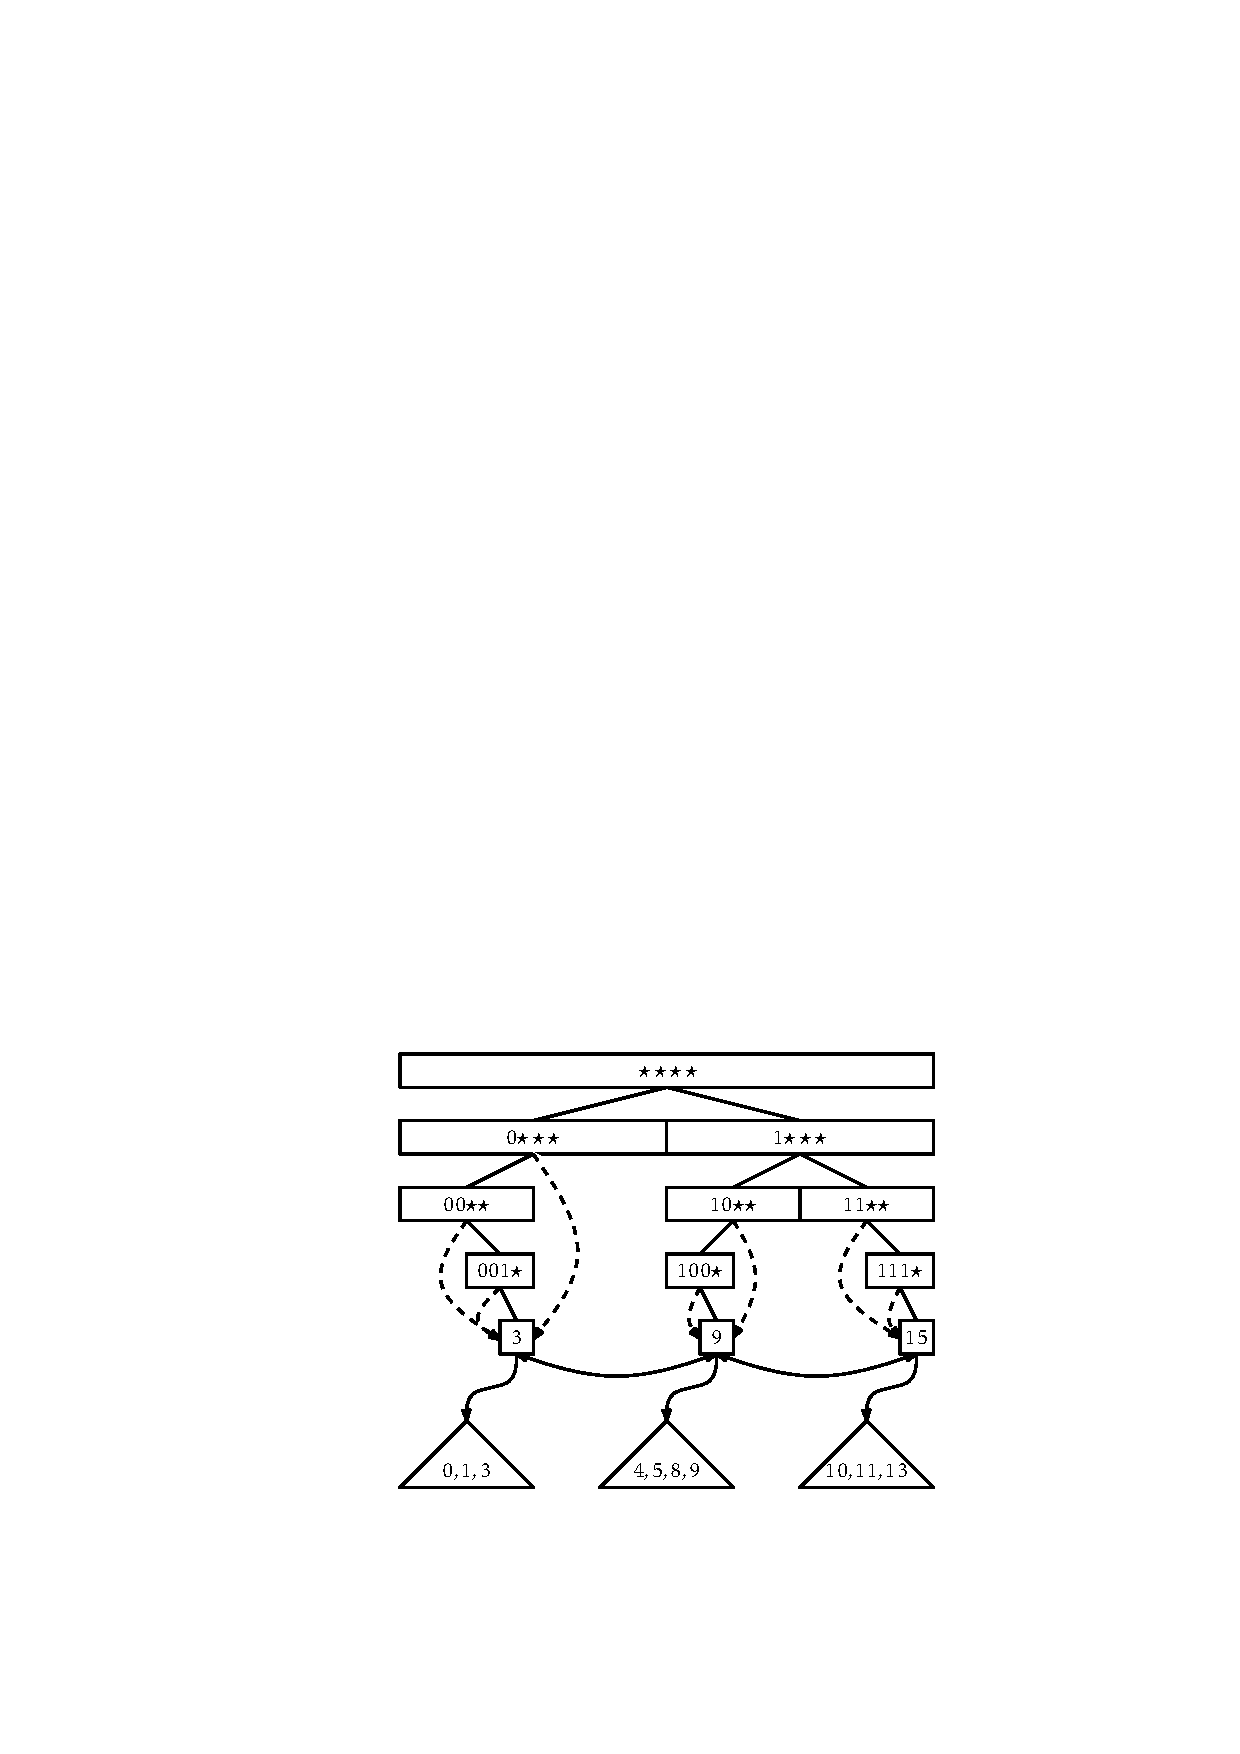
\includegraphics[scale=0.90909]{figs/yfast}
  \end{center}
  \caption[Uma YFastTrie]{Uma #YFastTrie# contendo os valores 0, 1, 3, 4,
  6, 8, 9, 10, 11, e 13.}
  \figlabel{yfast}
\end{figure}

A operação #find(x)# em uma #YFastTrie# é bastante fácil. Procuramos por #x# em #xft# e encontramos algum valor $#x#_i$ associado ao treap $#t#_i$. Em seguida, usamos o método da treap #find(x)# em $#t#_i$ para responder à consulta. Todo o método é de uma linha:
\codeimport{ods/YFastTrie.find(x)} 
A primeira operação #find(x)# (em #xft#) leva um tempo $O(\log#w#)$.
A segunda operação #find(x)# (em uma treap) leva um tempo $O(\log r)$, onde $r$ é o tamanho da treap. Posteriormente nesta seção, mostraremos que o tamanho esperado da treap é $O(#w#)$, de modo que esta operação leva um tempo $O(\log#w#)$.\footnote{Esta é uma aplicação da \emph {Desigualdade de Jensen}: Se $\E[r]=#w#$, então $\E[\log r]
\le \log w$.}

Adicionar um elemento a uma #YFastTrie# também é bastante simples --- na maioria das vezes. O método #add(x)# chama #xft.find(x)# para localizar a treap, #t#, na qual #x# deve ser inserido. Em seguida, chama #t.add(x)# para adicionar #x# a #t#. Nesse ponto, ele lança uma moeda tendenciosa que sai cara com probabilidade $1/#w#$ e coroa com probabilidade $1-1/#w#$.
Se esta moeda der cara, então #x# será adicionado a #xft#.

É aqui que as coisas ficam um pouco mais complicadas. Quando #x# é adicionado à #xft#, a treap #t# precisa ser dividida em duas treaps, #t1# e #t'#.
A treap #t1# contém todos os valores menores ou iguais a #x#; #t'# é a treap original, #t#, com os elementos de #t1# removidos.
Feito isso, adicionamos o par #(x,t1)# a #xft#. A \figref{yfast-add} mostra um exemplo.
\codeimport{ods/YFastTrie.add(x)}
\begin{figure}
  \begin{center}
    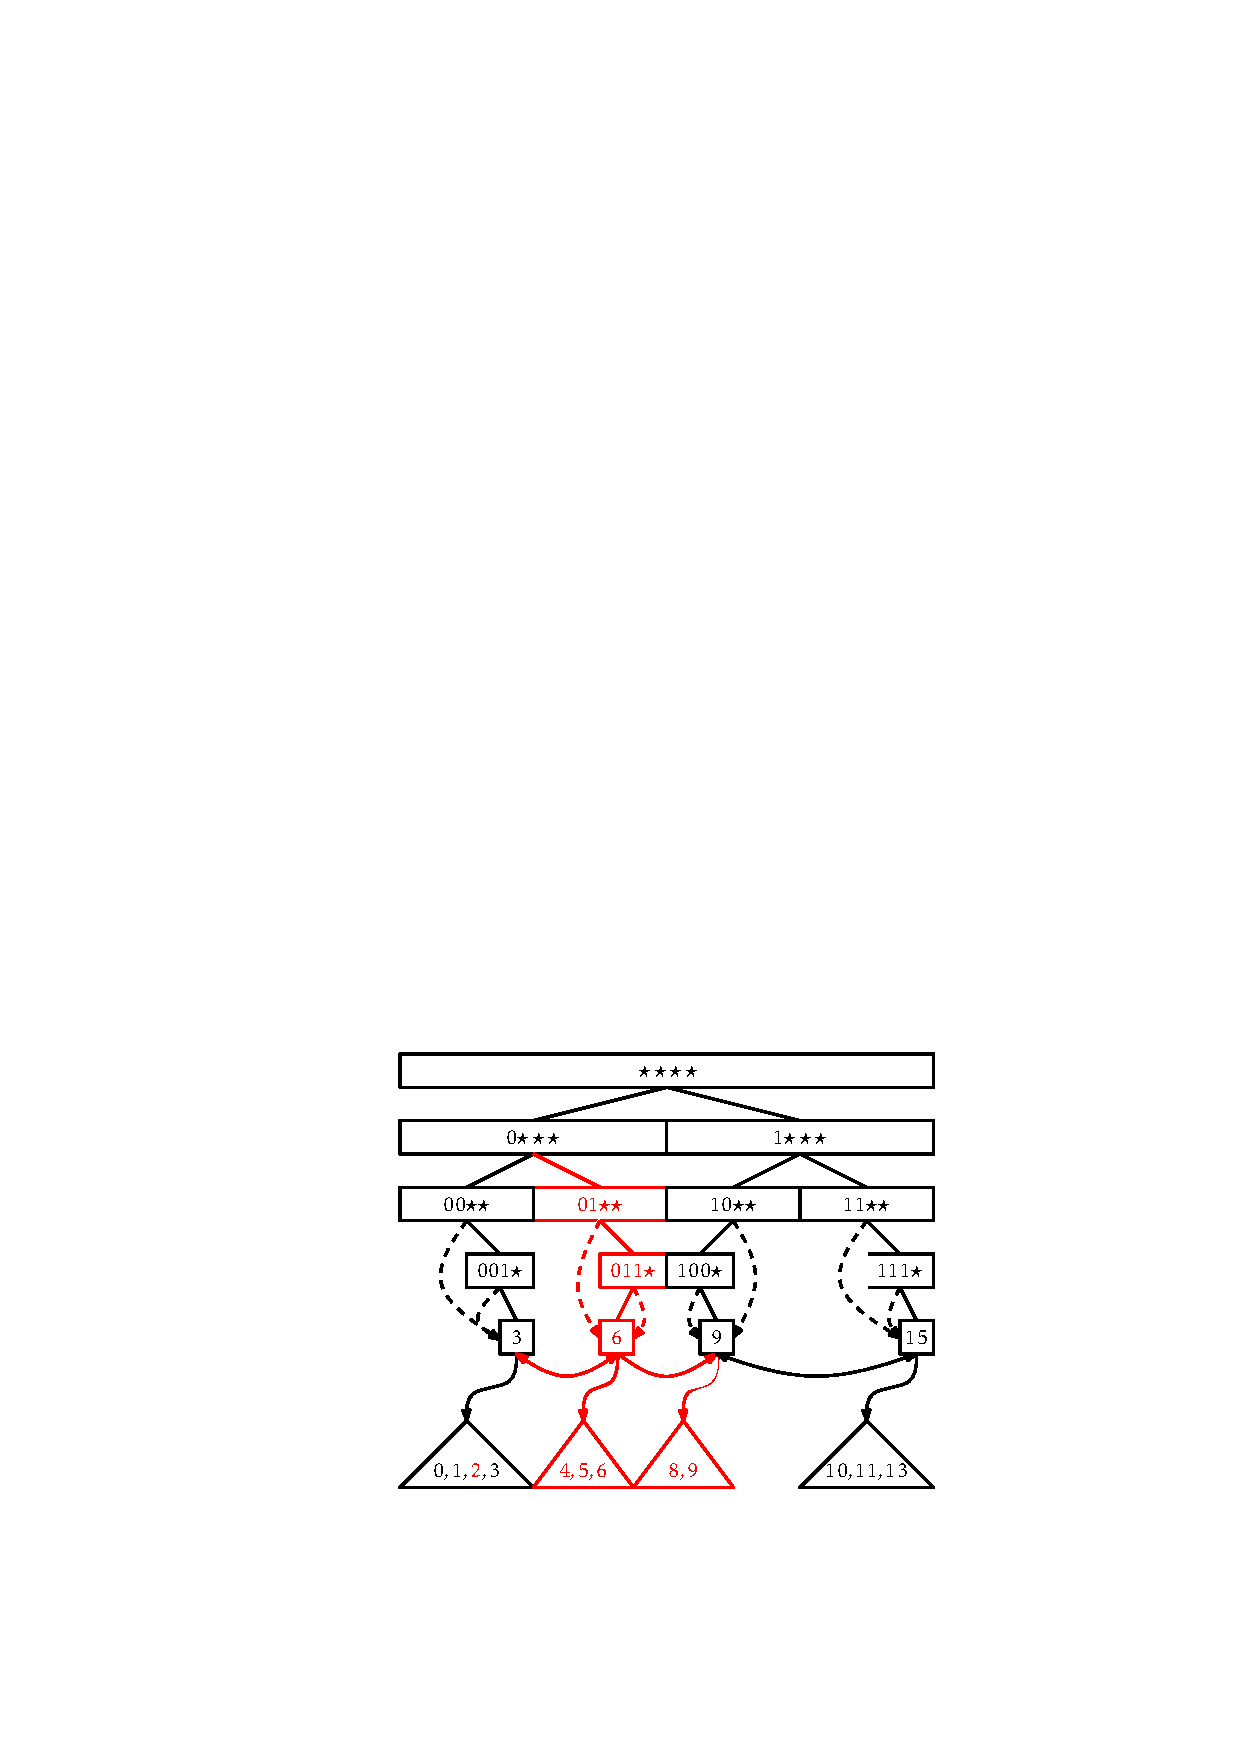
\includegraphics[scale=0.90909]{figs/yfast-add}
  \end{center}
  \caption[Adicionando a uma YFastTrie]{Adicionando os valores 2 e 6 a uma #YFastTrie#. O sorteio de 6 deu cara, então 6 foi adicionado à #xft# e a treap contendo $4,5,6,8,9$ foi dividida.}
  \figlabel{yfast-add}
\end{figure}
Adicionar #x# a #t# leva um tempo $O(\log #w#)$. \excref{treap-split} mostra que dividir #t# em #t1# e #t'# também pode ser feito em um tempo esperado de $O(\log #w#)$. Adicionar o par (#x#, #t1#) a #xft# leva um tempo $O(#w#)$, mas só acontece com a probabilidade $1/#w#$. Portanto, o tempo de execução esperado da operação #add(x)# é
\[
    O(\log#w#) + \frac{1}{#w#}O(#w#) = O(\log #w#) \enspace .
\]

O método #remove(x)# desfaz o trabalho executado por #add(x)#.
Usamos #xft# para encontrar a folha, #u#, em #xft# que contém a resposta para #xft.find(x)#. De #u#, obtemos a treap, #t#, contendo #x# e removemos #x# de #t#. Se #x# também foi armazenado em #xft# (e #x# não é igual a $2^{#w#}-1$), então removemos #x# de #xft# e adicionamos os elementos da treap de #x# à treap, #t2#, que é armazenada pelo sucessor de #u# na lista encadeada. Isso é ilustrado em
\figref{yfast-remove}.
\codeimport{ods/YFastTrie.remove(x)}
\begin{figure}
  \begin{center}
    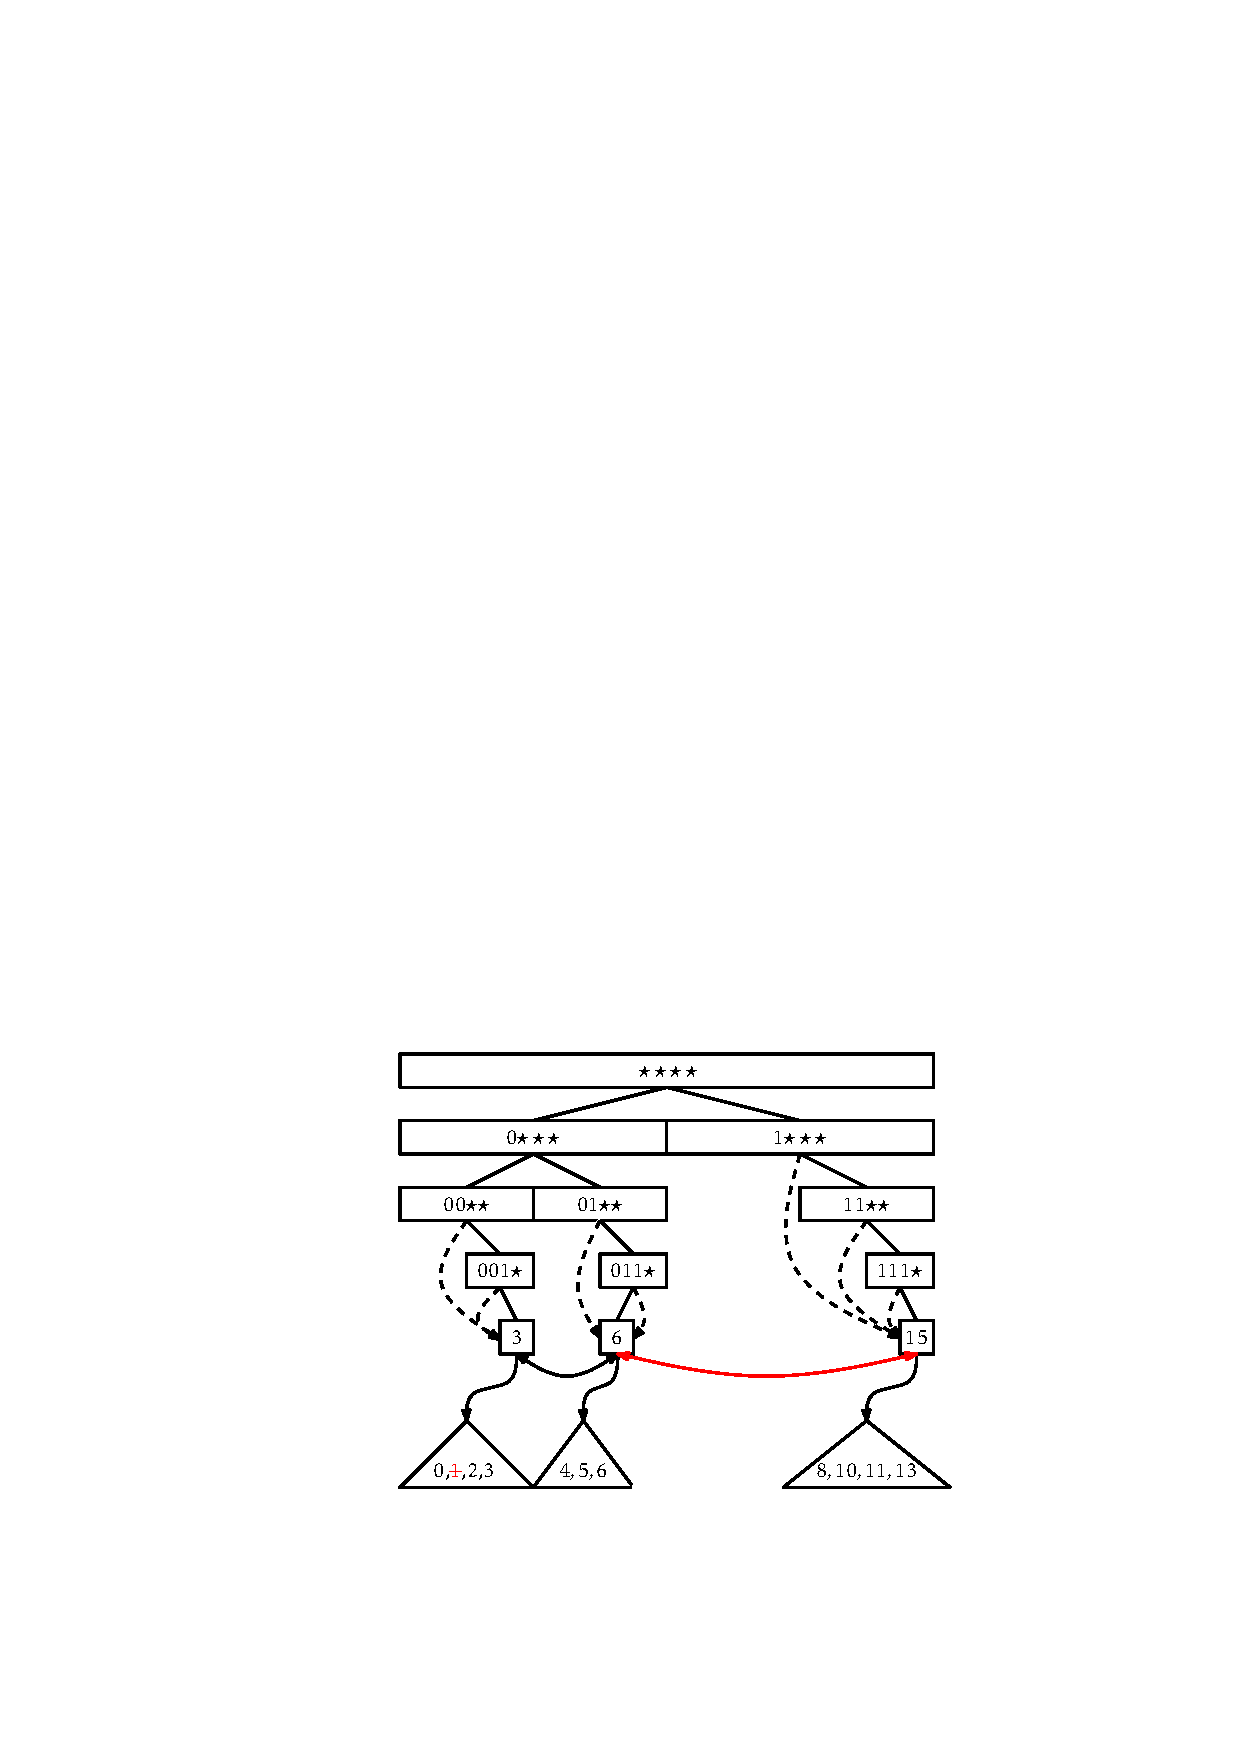
\includegraphics[scale=0.90909]{figs/yfast-remove}
  \end{center}
  \caption[Removendo de uma YFastTrie]{Removendo os valores 1 e 9 de uma #YFastTrie# na \figref{yfast-add}.}
  \figlabel{yfast-remove}
\end{figure}
Encontrar o nó #u# em #xft# leva um tempo esperado de $O(\log #w#)$.
Remover #x# de #t# leva um tempo esperado $O(\log #w#)$. Novamente, o \excref{treap-split} mostra que mesclar todos os elementos de #t# em #t2# pode ser feito em tempo $O(\log #w#)$. Se necessário, remover #x# de #xft# leva um tempo $O(#w#)$, mas #x# só está contido em #xft# com probabilidade $1/#w#$. Portanto, o tempo esperado para remover um elemento de uma #YFastTrie# é $O(\log #w#)$.

No início da discussão, atrasamos a discussão sobre os tamanhos das treaps nesta estrutura para mais tarde. Antes de terminar este capítulo, provamos o resultado de que precisamos.

\begin{lem}\lemlabel{yfast-subtreesize}
Seja #x# um inteiro armazenado em uma #YFastTrie# e seja $#n#_#x#$ o número de elementos na treap, #t#, que contém #x#.
Então $\E[#n#_#x#] \le 2#w#-1$.
\end{lem}

\begin{proof}
Referir-se à \figref{yfast-sample}. Seja
$#x#_1<#x#_2<\cdots<#x#_i=#x#<#x#_{i+1}<\cdots<#x#_#n#$
os elementos armazenados na #YFastTrie#. 
A treap #t# contém alguns elementos maiores ou iguais a #x#.  Esses são $#x#_i,#x#_{i+1},\ldots,#x#_{i+j-1}$,
onde $#x#_{i+j-1}$ é o único desses elementos em que o lance de moeda tendencioso realizado no método #add(x)# deu cara.
Em outras palavras, $\E[j]$ é igual ao número esperado de lançamentos tendenciosos de moeda necessários para obter as primeiras caras.\footnote {Esta análise ignora o fato de que $j$ nunca excede $#n#-i+1$. No entanto, isso apenas diminui $\E[j]$, então o limite superior ainda se mantém.} Cada sorteio é independente e sai cara com probabilidade $1/#w#$, então $\E[j]\le#w#$.
(Veja \lemref{coin-tosses} para uma análise disto para o caso $#w#=2$.)

Da mesma forma, os elementos de #t# menores que #x# são
$#x#_{i-1},\ldots,#x#_{i-k}$ onde todos esses $k$ lançamentos de moeda resultam em coroa e o lançamento de $#x#_{i-k-1}$ dá cara. Portanto, $\E[k]\le#w#-1$, já que este é o mesmo experimento de lançamento de moeda considerado no parágrafo anterior, mas aquele em que o último lançamento não é contado.
Em resumo, $#n#_#x#=j+k$, então
\[  \E[#n#_#x#] = \E[j+k] = \E[j] + \E[k] \le 2#w#-1 \enspace .  \qedhere \]
\end{proof}
\begin{figure}
  \begin{center}
    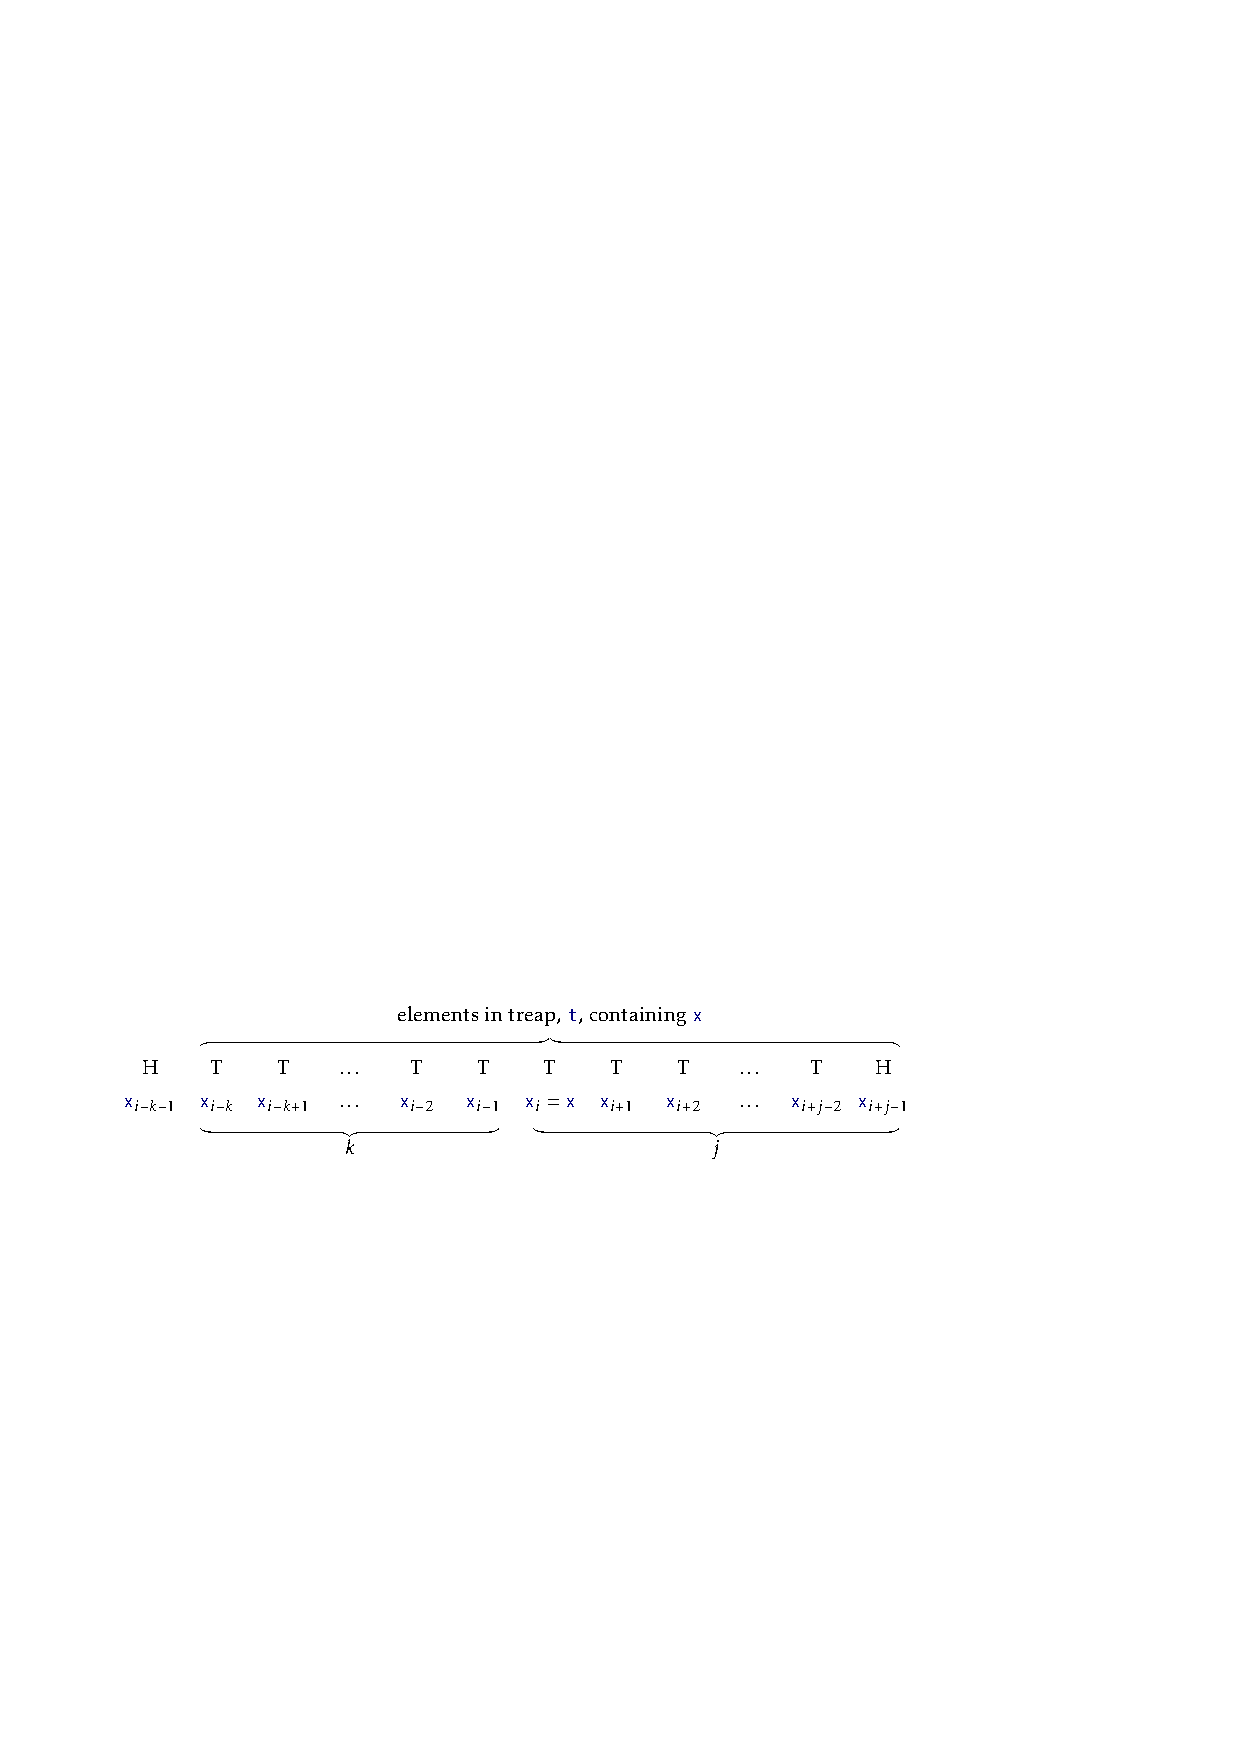
\includegraphics[width=\ScaleIfNeeded]{figs/yfast-sample}
  \end{center}
  \caption[O tempo de consulta em uma YFastTrie]{O número de elementos na treap #t# contendo #x# é determinado por dois experimentos de lançamento de moeda.}
  \figlabel{yfast-sample}
\end{figure}
%Surprisingly, the bound in \lemref{yfast-subtreesize} is tight.  (If this
%isn't surprising to the reader, they can stop reading this paragraph now.)
%This is counterintuitive because #xft# contains any particular element
%with probability $1/#w#$ so it contains about $n/#w#$ elements.  In other
%words, the average number of elements assigned to one treap is #w#.
%\lemref{yfast-subtreesize} says that the expected size of the treap that
%contains #x# is about twice as large as the average.  This seeming
%discrepancy comes from the fact that larger subtrees contain more elements
%and therefore #x# is more likely to be in a larger subtree than a smaller
%one.

\lemref{yfast-subtreesize} foi a última peça na prova do seguinte teorema, que resume o desempenho da #YFastTrie#:

\begin{thm}
Uma #YFastTrie# implementa a interface #SSet# para inteiros de #w#-bits. Uma #YFastTrie# suporta as operações #add(x)#, #remove(x)# e #find(x)# em tempo esperado de $O(\log#w#)$  por operação. O espaço usado por uma #YFastTrie# que armazena #n# valores é $O(#n#+#w#)$.
\end{thm}

O termo #w# no requisito de espaço vem do fato de que #xft# sempre armazena o valor $2^#w#-1$. A implementação pode ser modificada (às custas de adicionar alguns casos extras ao código) para que seja desnecessário armazenar esse valor. Neste caso, o requisito de espaço no teorema torna-se $O(#n#)$.

\section{Discussão e Exercícios}

A primeira estrutura de dados a fornecer operações #add(x)#, #remove(x)# e #find(x)# em um tempo $O(\log#w#)$ foi proposta por van~Emde~Boas e desde então tornou-se conhecida como o \emph{árvore van~Emde~Boas}
\index{arvore@árvore van Emde Boas}%
(ou \emph{estratificada})
\index{arvore@árvore estratificada}%
\cite{e77}.  A estrutura original de van~Emde~Boas tinha tamanho
$2^{#w#}$, tornando-a impraticável para números inteiros grandes.

As estruturas de dados #XFastTrie# e #YFastTrie# foram descobertas por Willard \cite{w83}. A estrutura #XFastTrie# está intimamente relacionada às árvores van~Emde~Boas; por exemplo, as tabelas de hash em uma #XFastTrie# substituem arrays em uma árvore van~Emde~ Boas. Ou seja, em vez de armazenar a tabela de hash #t[i]#, uma árvore van~Emde~Boas armazena uma matriz de comprimento $2^{#i#}$.

Outra estrutura para armazenar inteiros são as árvores de fusão de Fredman e Willard \cite{fw93}.
\index{arvore@árvore de fusão}%
Esta estrutura pode armazenar #n# inteiros de #w# bits em um espaço
$O(#n#)$ de modo que a operação #find(x)# execute em um tempo $O((\log #n#)/(\log
#w#))$.  Usando uma árvore de fusão quando $\log #w#>\sqrt{\log #n#}$ e uma #YFastTrie# quando $\log#w#\le \sqrt{\log #n#}$, obtém-se uma estrutura de dados de espaço $O(#n#)$ que pode implementar a operação #find(x)# em tempo $O(\sqrt{\log #n#})$. Resultados recentes de limite inferior de P\v{a}tra\c{s}cu e Thorup \cite{pt07} mostram que esses resultados são mais ou menos ideais, pelo menos para estruturas que usam apenas espaço $O(#n#)$.

\begin{exc}
  Projete e implemente uma versão simplificada de uma #BinaryTrie# que não tenha uma lista encadeada ou ponteiros de salto, mas para o qual #find(x)# ainda é executado em tempo $O(#w#)$.
\end{exc}

\begin{exc}
  Projete e implemente uma implementação simplificada de uma #XFastTrie# que não use um teste binário. Em vez disso, sua implementação deve armazenar tudo em uma lista duplamente encadeada e $#w#+1$ tabelas de hash.
\end{exc}

\begin{exc}
  Podemos pensar na #BinaryTrie# como uma estrutura que armazena sequências de bits de comprimento #w# de forma que cada sequência de bits seja representada como um caminho da raiz para folha. Estenda essa ideia em uma implementação #SSet# que armazena strings de comprimento variável e implementa #add(s)#, #remove(s)# e #find(s)# no tempo proporcional ao comprimento de #s#.

  \noindent Dica: Cada nó em sua estrutura de dados deve armazenar uma tabela hash que é indexada por valores de caractere.
\end{exc}

\begin{exc}
  Para um inteiro $#x#\in\{0,\ldots2^{#w#}-1\}$, faça $d(#x#)$ denotar a diferença entre #x# e o valor retornado por #find(x)# [se #find(x)# retorna #null#, então defina $d(#x#)$ como $2^#w#$].
  Por exemplo, se #find(23)# retorna 43, então $d(23)=20$.
  \begin{enumerate}
    \item Projete e implemente uma versão modificada da operação #find(x)# em uma #XFastTrie# executada em tempo esperado de $O(1+\log d(#x#))$. Dica: a tabela hash $t[#w#]$ contém todos os valores, #x#, de forma que $d(#x#)=0$, então esse seria um bom lugar para começar.
    \item Projete e implemente uma versão modificada da operação #find(x)# em uma #XFastTrie# executada em um  tempo esperado de $O(1+\log\log d(#x#))$.
  \end{enumerate}
\end{exc}


